\chapter{Applications of HT-smFRET}
\label{chpt:HT-smFRET_applications}

The potential of the \ac{HT-smFRET} setup is exciting, especially in the context of current \ac{smFRET} applications, which are typically only capable of equilibrium measurements.
Here, I first describe equilibrium measurements performed on the 48-spot setup for the purpose of characterization of the new instrument.
Then I present kinetic studies performed on the 8-spot setup to demonstrate the exciting possibilities of \ac{HT-smFRET} for non-equilibrium studies of freely-diffusing biological systems.
Finally, I present the results of a proof of principle experiment where I incorporated a simple microfluidic device to the 48-spot setup and demonstrate \ac{HT-smFRET} on a flowing sample.
Together, these works outline a pathway to achieving time-resolved \ac{smFRET} experiments on non-equilibrium systems, opening the exciting possibility of observing precise distances changes on entire kinetic trajectories.

\section{Equilibrium smFRET measurements}
\label{sec:HT-smFRET_measurements}

In order to characterize the 48-spot setup, I first performed equilibrium \ac{smFRET} measurements on doubly-labeled \ac{dsDNA}.
The following section provides a detailed account of theses experiments and their analysis.

\subsection{HT-smFRET-PAX of freely diffusing dsDNA}
\label{sec:HT-smFRET_measurements_DNA}

To showcase the enhanced throughput of the 48-spot smFRET-PAX setup, I initially conducted measurements using doubly-labeled \ac{dsDNA}. These samples were 40~\ac{bp}s long and were designed to be identical expect for the location of the dyes.  
Each sample was labeled with ATTO550 as the donor dye and ATTO647N as the acceptor dye, with different samples characterized by varying inter-dye distances, as explained in previous work~\cite{ingargiola_PLOS1_2016}. 
In this study, I used two samples with inter-dye distances of 12~\ac{bp} and 22~\ac{bp}\cite{ingargiola_JCP_2018}. 
The measurements were carried out on samples with a nominal concentration of 100 pM in TE 50 buffer, a minimal DNA storage buffer containing 10~mM Tris (pH = 8.0), 1~mM EDTA, and 50~mM NaCl. 
First, I performed measurements using a standard single-spot \ac{ALEX} setup. 
Then, I measured the exact same samples with the 48-spot PAX setup.
This approach ensured that the sample conditions were consistent for a meaningful comparison of the setup characteristics.

\subsection{Burst search and selection}
\label{sec:burst_search_and_selection_PAX_analysis}

I conducted the \ac{smFRET} analysis in three distinct steps.
A detailed explanation of each step can be found in the  Appendix~\ref{chpt:analysis_appendix}:

\begin{enumerate}
\item Background estimation
\item Burst search
\item Burst selection
\end{enumerate}

To address potential background fluctuations, I estimated the background rate for each photon stream at each spot using a 10 second moving time window. 
Following this, I conducted an \ac{APBS} for each spot using the standard sliding window algorithm. 
This approach involved defining the local total count rate based on 10 consecutive photons ($m=10$) and employing a fixed threshold to delineate burst start and end points (set at $50\times 10^{3}$ counts per second or 50~kHz).

After the burst search, I applied various selection criteria to isolate specific burst subpopulations. 
Typically, I initiated a preliminary burst selection based on a minimum background-corrected total count (\textit{e.g.}, $\geq 30$ photons) to retain bursts with a sufficient signal-to-noise ratio. 
Additionally, further selections were employed to distinguish FRET species from donor-only and acceptor-only molecules. 
This differentiation was achieved by choosing bursts with a total background corrected acceptor signal ($\overline{F}_{DA_{ex}A_{em}}$) greater than a defined minimum value, as shown in Figure~\ref{fig:48-spot_FRET_pop}. 
However, to identify and visually select subpopulations, I often utilized the 2D $E-S$ histogram, which is discussed in the next Section~\ref{sec:Epr_Su_PAX} and in more depth in Appendix~\ref{sec:E_S_histogram}.

\subsection{$E - S$ histograms for HT-smFRET-PAX}
\label{sec:Epr_Su_PAX}

Following burst selection, I generated a 2D histogram of $E$ and $S$, where $E$ represents the FRET efficiency, and $S$ denotes the stoichiometry ratio as defined in Appendix~\ref{sec:E_S_histogram}. 
Here, $S$ can be approximated as $N_D / (N_D + N_A)$, where $N_D$ and $N_A$ represent the respective counts of donor and acceptor molecules within a burst.

In practical terms, the exact calculation of corrected $E$ and $S_{\gamma\beta}$ values necessitates knowledge of various correction factors that might not be available at the outset of the analysis, see Appendix~\ref{sec:Epr_apdx} and \ref{sec:correction_factors} for more details. 
Rather than plot the corrected values, we utilized the related, uncorrected quantities, $E_{PR}$ and $S$ (or the \ac{PAX}-specific $S_u$), that are simpler to compute.
These quantities are defined in Appendix~\ref{sec:ratiometric_E_S_apdx}). 
These alternative values enabled the identification of different sub-populations. 
We generated corresponding 2D histograms of $E_{PR}$ and $S$, or $S_u$, which facilitated the separation of FRET species from singly labeled donor-only or acceptor-only species, as demonstrated in Fig.~\ref{fig:48-spot_FRET_pop}.

\begin{figure}
\centering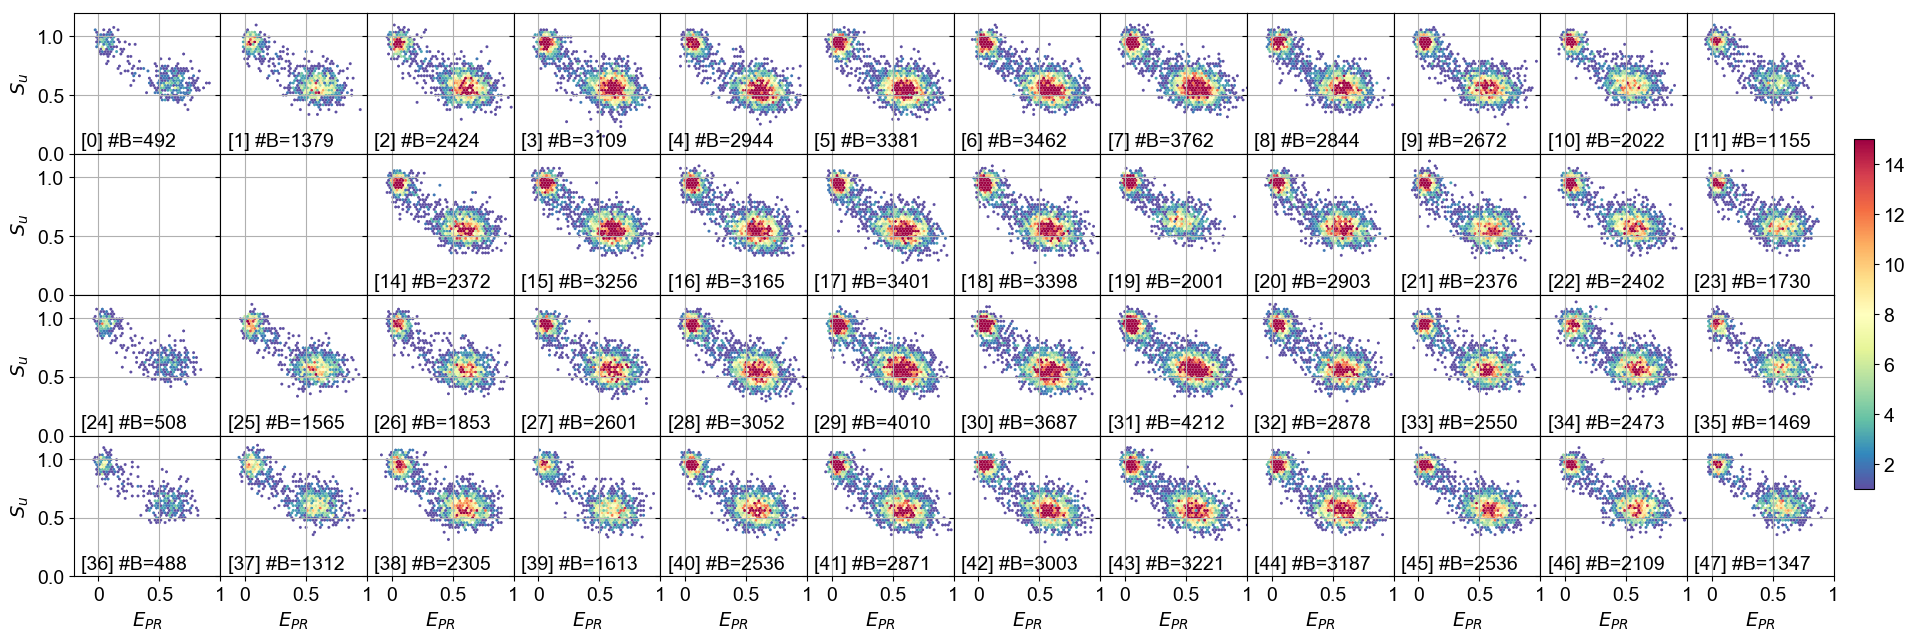
\includegraphics[width=1.0\linewidth]{chapters/figures/2017-05-23_08_12d_48spot_alex_hist_Su_all-bursts.png}
\caption{\label{fig:48-spot_FRET_pop} $E_{PR} - S_u$ histograms for each 
spot from a doubly-labeled \ac{dsDNA} sample with a 12~\ac{bp} inter-dye separation. 
A burst search using all photons (\ac{APBS}) was preformed, with $m=10$ and a constant threshold of 50~kHz.
After background correction, bursts were selected using a minimum burst size of 40~photons.
The total number of bursts is indicated as $\#B$ at the bottom of each histogram.  
The 12~\ac{bp} FRET population ($E_{PR} \approx 0.6, S_u \approx 0.6$) is isolated from donor-only or acceptor-only populations.
Spots 12 and 13 correspond to two defective pixels in the donor \ac{SPAD} array.
For computational details refer to the \texttt{48-spot-smFRET-PAX-analysis}  
\href{https://github.com/tritemio/48-spot-smFRET-PAX-analysis}{notebooks}.
Figure reproduced from the original 48-spot publication~\cite{ingargiola_JCP_2018}.
}
\end{figure}

Accuracy of the multispot data analysis was verified by comparing the results obtained for each spot. 
By applying a second burst selection criterion, $\overline{F}_{DA_{ex}A_{em}} > \text{min}$, we effectively eliminated the donor-only population and isolated the FRET subpopulations as visualized in Fig.~\ref{fig:48-spot_FRET_pop}. 

Subsequently, fitting the burst distribution of these subpopulations with a 2D Gaussian enabled us to determine their center-of-mass and standard deviation. 
These parameters are depicted in Figure~\ref{fig:peak_Epr_S}A as blue dots and crosses, respectively. 
The orange dot in Figure~\ref{fig:peak_Epr_S}A represents the average position of the FRET peak across all spots. 

It is noteworthy that even without spot-specific corrections, the overall dispersion of these populations remains minimal.
This is evident in scatterplot of the FRET population (blue pluses in Figure~\ref{fig:peak_Epr_S}B) and the donor-only population (orange crosses in Figure~\ref{fig:peak_Epr_S}B).

\begin{figure}
\centering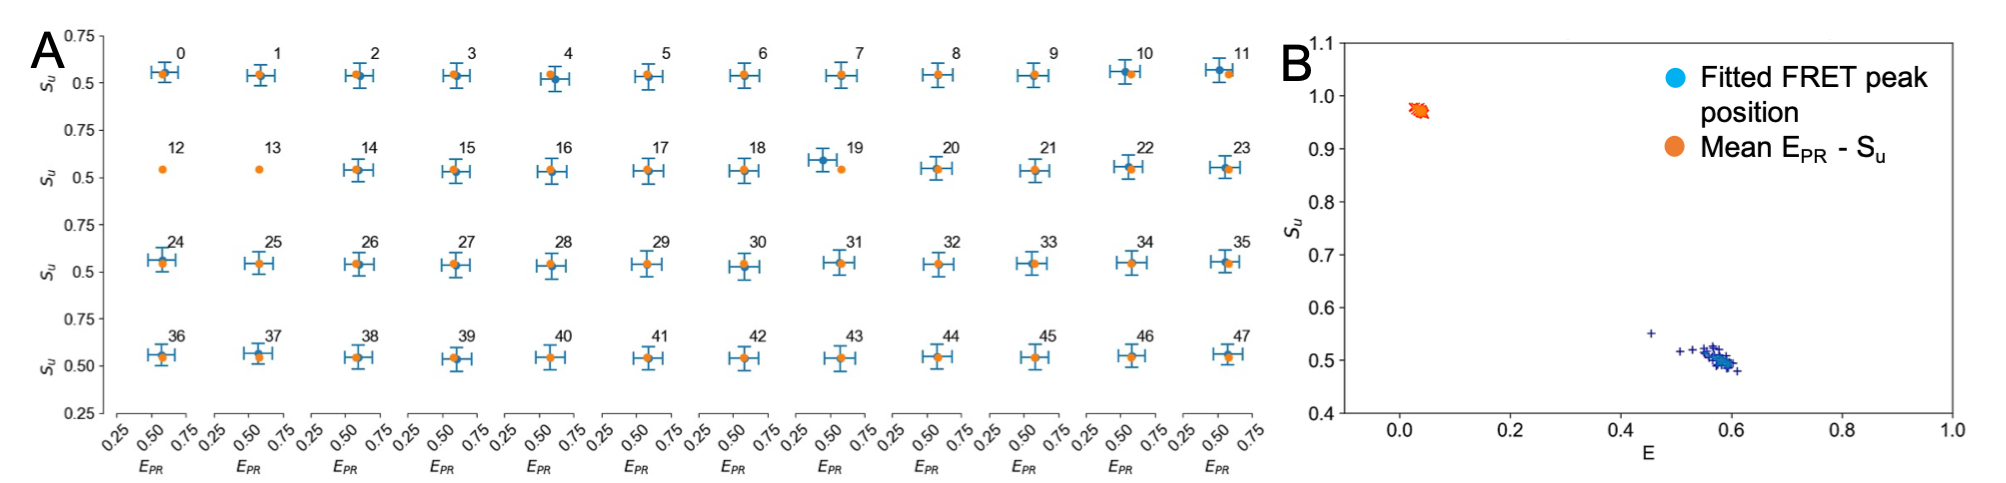
\includegraphics[width=1.0\linewidth]{chapters/figures/Epr_Su_peaks.png} 
\caption{\label{fig:peak_Epr_S}
A) Gaussian fitted $E_{PR} - S_u$ peak position for each spot.
FRET peak positions and standard deviations are denoted by blue dots and crosses respectively. 
Spots 12 and 13 correspond to two defective pixels in the donor \ac{SPAD} array.
B) FRET (blue pluses) and donor-only (orange crosses) peak position for all spots. 
For computational details refer to the \texttt{48-spot-smFRET-PAX-analysis} 
\href{https://github.com/tritemio/48-spot-smFRET-PAX-analysis}{notebooks}.
Figure adapted from the original 48-spot publication~\cite{ingargiola_JCP_2018}.}
\end{figure}

\subsection{Pooling data from HT-smFRET-PAX measurements}
\label{sec:pooling_data}

The last stage of \ac{HT-smFRET}-PAX analysis consists of pooling data from all spots into a unified global dataset. 
To address any variations between spots, we applied spot-specific $\gamma$ and $\beta$ corrections, as detailed in Appendix~\ref{sec:E_apdx} and ~\ref{sec:S_apdx}. 
Figure~\ref{fig:pooled_mixed} illustrates the outcome of this procedure using data obtained from a mixture of doubly-labeled \ac{dsDNA} with inter-dye distances of 12~\ac{bp} and 22~\ac{bp}.

\begin{figure}
\centering
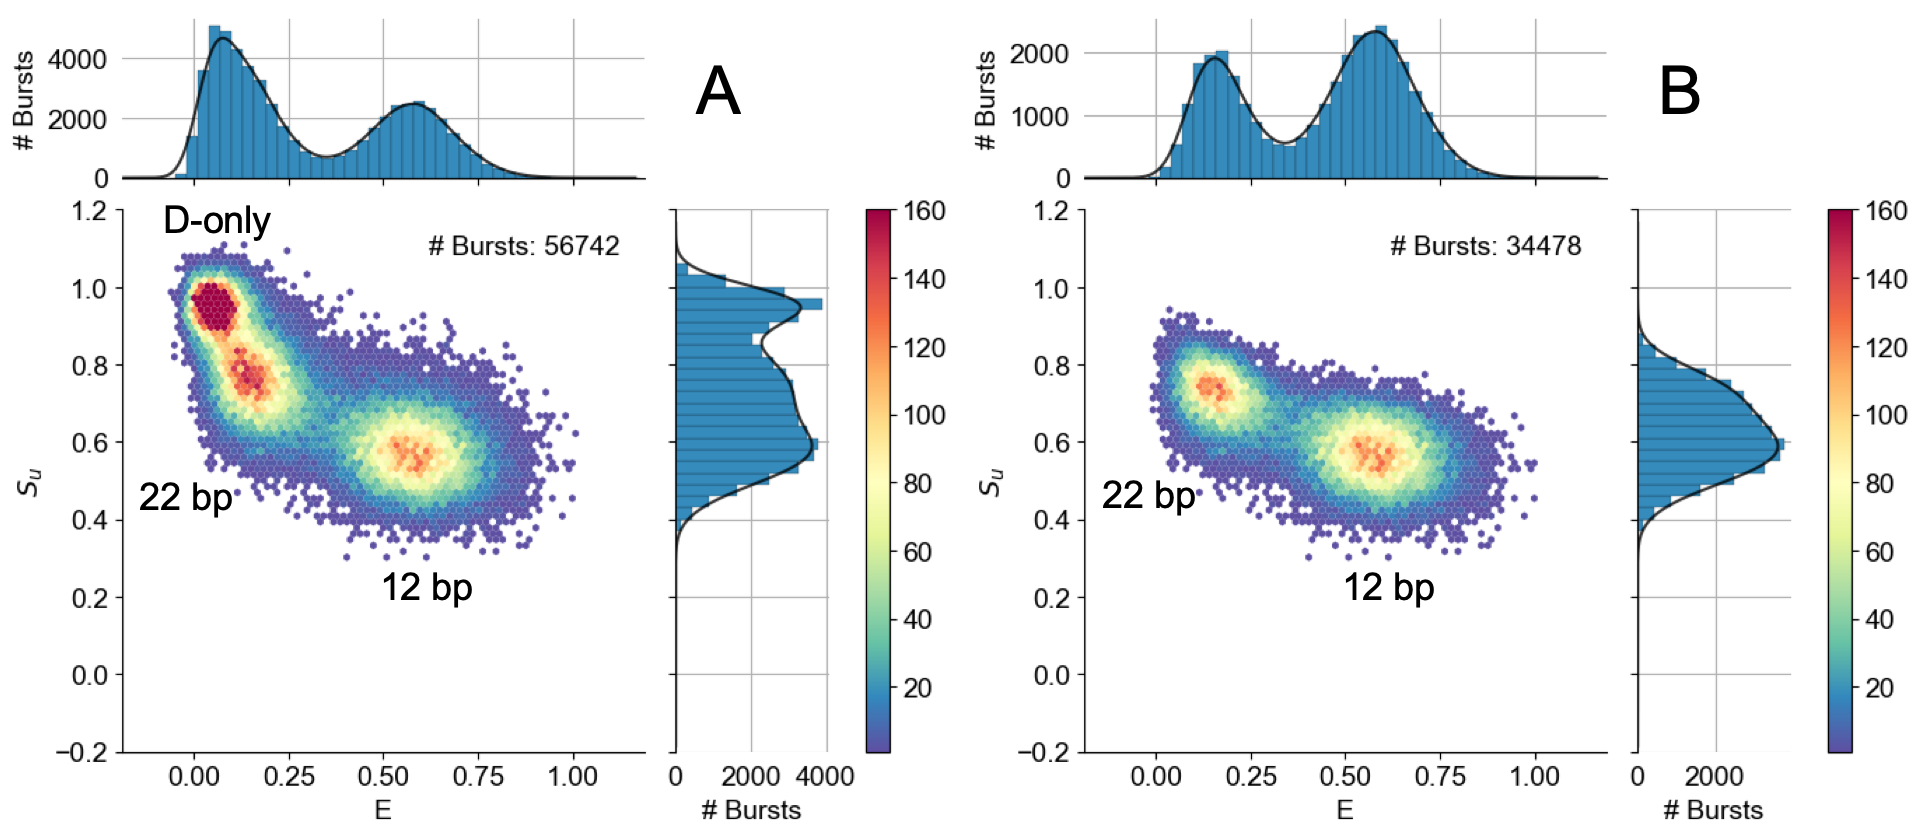
\includegraphics[width=1.0\linewidth]{chapters/figures/pooled_mixed-pop.png}
\caption{\label{fig:pooled_mixed} 
Pooled data from \ac{HT-smFRET}-PAX measurements of freely diffusing dsDNA separated by 12~\ac{bp} and 22~\ac{bp}, where $\gamma= 0.5$ for the multispot-PAX setup. 
No spot-specific corrections were applied. 
A) Burst search using $m = 10$ and a constant rate threshold of 50~kHz, burst size selection using  $> 80$ photons. 
B) Histogram from A) with an additional burst selection, $\overline{F}_{DA_{ex}A_{em}} > 25$ photons. 
The additional selection removes the donor-only population from the histogram and leaves two FRET subpopulations 
corresponding to the 12~\ac{bp} and 22~\ac{bp} FRET species.
For computational details refer to the \texttt{48-spot-smFRET-PAX-analysis} \href{https://github.com/tritemio/48-spot-smFRET-PAX-analysis}{notebooks}.
Figure adapted from the original 48-spot publication~\cite{ingargiola_JCP_2018}.}
\end{figure}

Pooling the bursts from all spots yields a substantial number of bursts, enabling the application of stricter selection criteria, such as a larger minimum burst size, to retain only those bursts with a robust signal-to-noise ratio. 
Furthermore, this data pooling allows for the extraction of sub-population information within a much shorter acquisition time compared to what could be achieved with a standard single-spot setup. 
This efficiency is demonstrated in Figure~\ref{fig:pooled_comparison}, where we aquired 5~s of data on a single-spot \ac{ALEX} setup and the 48-spot \ac{PAX} setup.

Pooling data from all 46 spots (with 2 \ac{SPAD}s being defective in one of the arrays) resulted in a 38-fold increase in the number of observed bursts compared to the single-spot experiment. 
Notably, this 38-fold increase varies at different observation time points due to the stochastic nature of single-molecule transit through the excitation-detection spots and differences in the excitation-detection volumes and detection efficiencies between the two setups.

\begin{figure}
\centering
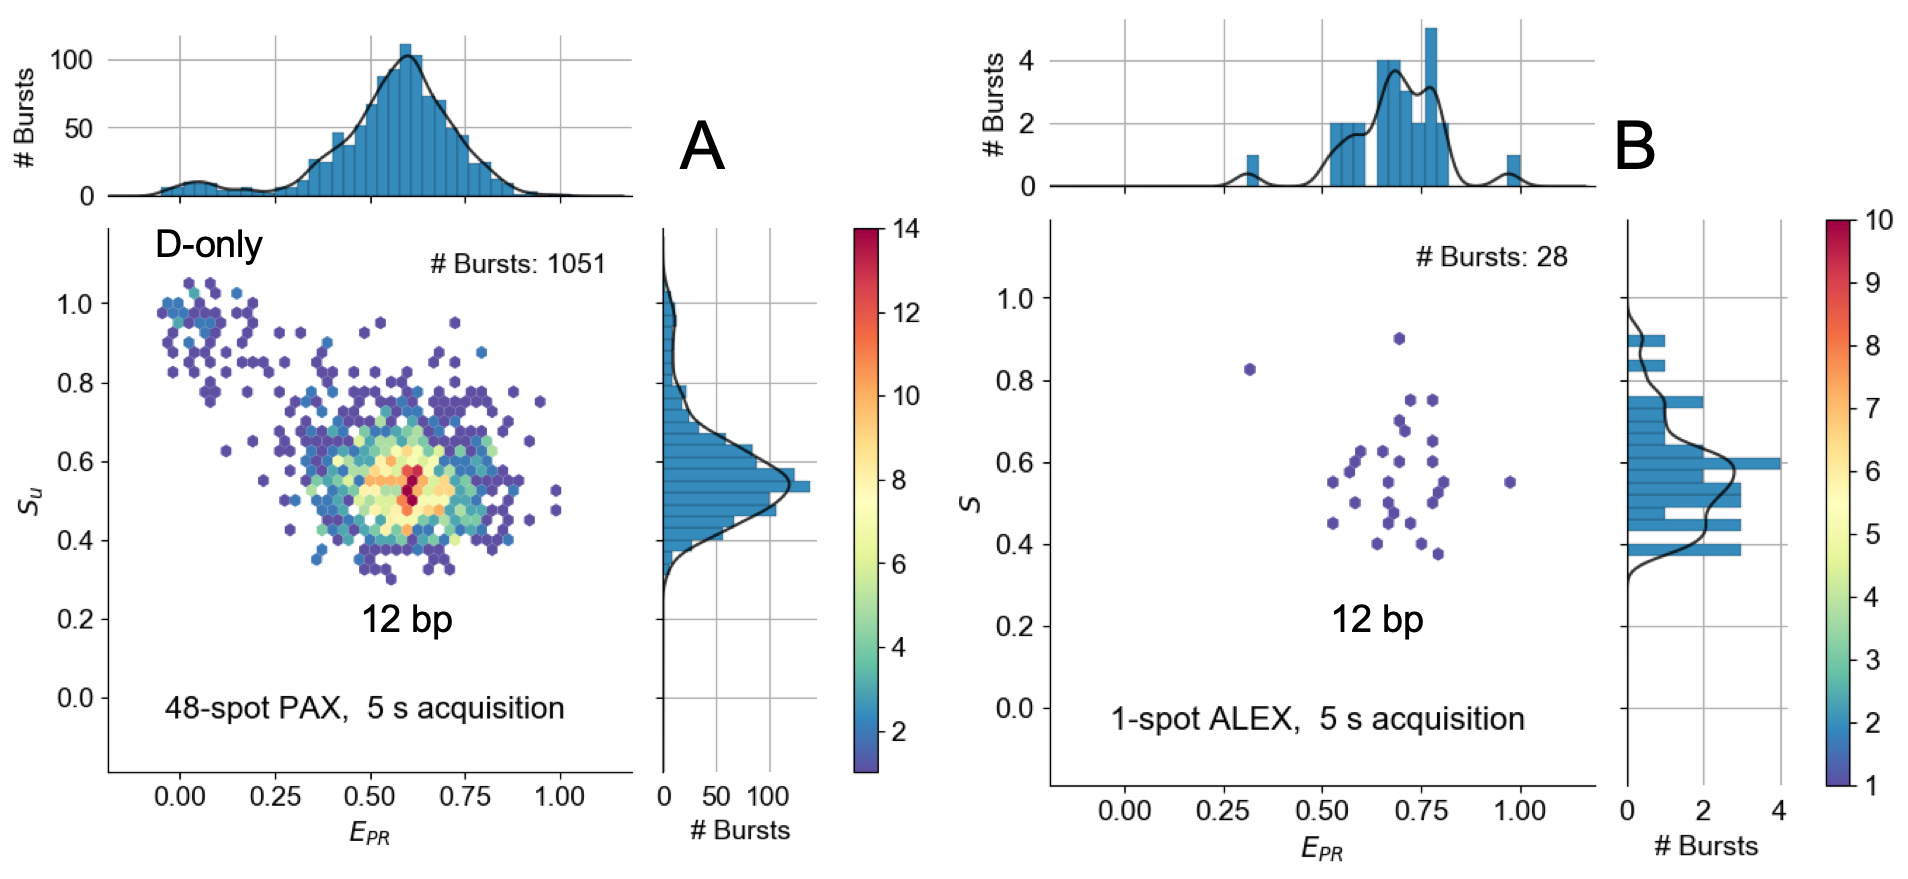
\includegraphics[width=1.0\linewidth]{chapters/figures/pooled_setup_comparison.png}
\caption{\label{fig:pooled_comparison} 
Pooled data from \ac{HT-smFRET}-PAX 
measurements of freely diffusing dsDNA separated by 12~\ac{bp}. 
Where $\gamma= 0.5$ for the \ac{PAX} setup. 
No per-spot corrections were applied. 
A) $E_{PR} - S_u$ histogram for 5~s of acquisition with the 48-spot setup. 
A constant rate threshold $= 20$~kHz was applied followed by a burst selection on the counts during
donor excitation, $\overline{F}_{D\gamma} > 20$. 
1,051 bursts were collected in 5~s. 
B) $E_{PR} - S$ histogram for 5~s of acquisition on the single-spot\ac{ALEX} setup using the same sample from A). 
A constant threshold $= 20$~kHz was applied followed by a burst selection on the counts during donor excitation, $\overline{F}_{D\gamma} > 20$.
Only 28 bursts were collected in 5~s. 
For computational details refer to the \texttt{48-spot-smFRET-PAX-analysis} 
\href{https://github.com/tritemio/48-spot-smFRET-PAX-analysis}{notebooks}.
Figure reproduced from the original 48-spot publication~\cite{ingargiola_JCP_2018}.}
\end{figure}

The improved throughput offers the potential to enhance the temporal resolution of out-of-equilibrium reaction studies, particularly in "standing drop" sample geometries where molecules diffuse in and out of the excitation-detection volumes. 
In theory, the temporal resolution of such measurements is inversely related to the burst rate, which represents the number of bursts detected per unit of time. 
However, it is important to note that this relationship holds true after the reaction has reached a steady state throughout the sampled volume, as is explained in greater depth in the next section.

\section{Kinetic study of bacterial transcription}

We employed our initial 8-spot setup to investigate the kinetics of transcription initiation by bacterial \ac{RNAP} as an illustration of \ac{HT-smFRET}, as detailed in the following section.

\subsection{Experimental details}
\label{sec:exp_details_RNAP_kinetics}

As described in detail in Section~\ref{sec:RNAP_cycle}, DNA transcription into RNA by \ac{RNAP} occurs in three main steps: i) initiation, ii) elongation, and iii) termination.

Transcription initiation is a highly regulated process and represents the rate-limiting step of the reaction, as indicated in previous studies~\cite{murakami_structural_2002}. 
This process involves four critical steps:


\begin{enumerate}
\item Binding of the core \ac{RNAP} to the promoter specificity $\sigma$ factor, resulting in the formation of the \ac{RNAP} holoenzyme.
\item Binding of the \ac{RNAP} holoenzyme to the DNA at the promoter sequence located upstream from the gene sequence. 
Resulting in formation of the RNAP-promoter closed bubble, \ac{$RP_c$}, complex.
\item A series of events leading to the unwinding of approximately 10-12~\ac{bp}s of the \ac{dsDNA} promoter sequence, leading to the creation of the RNAP-promoter open bubble, \ac{$RP_o$}, complex.
\item Initiation of RNA polymerization, which involves numerous unsuccessful attempts (abortive initiation). 
Eventually, this leads to promoter escape and the transition to the elongation phase.
\end{enumerate}

The open bubble formed during transcription initiation can be stabilized by introducing a dinucleotide, resulting in the formation of what is referred to as the $RP_{ITC = 2}$ intermediate complex (see Figure~\ref{fig:RNAP_kinetics}A). This $RP_{ITC = 2}$ complex remains stable until the addition of \ac{NTP}s, which are essential for the transcription of the gene~\cite{lerner_PNAS_2016}.

The transcription reaction begins with the introduction of all four \ac{NTP}s: ATP, UTP, GTP, and CTP into the assay. 
This reaction continues until a full-length RNA is synthesized, and the \ac{dsDNA} of the promoter region is restored to a closed formation.
This process is referred to as termination and is depicted in Figure ~\ref{fig:RNAP_kinetics}B.

To investigate the kinetics of the transition from initiation to termination, we monitored the FRET efficiency between two labeled nucleotides located on opposite strands of DNA within the bubble region. 
Specifically, we examined the changes in FRET between the template strand (donor-labeled with ATTO~550) and the non-template strand (acceptor-labeled with ATTO~647N).

In the initiation stage, prior to the addition of \ac{NTP}s (i.e., the $RP_{ITC=2}$ stage), the dyes are separated, leading to a medium FRET efficiency. 
However, as \ac{RNAP} moves along the DNA during elongation, the DNA strands at the promoter sequence re-anneal, causing a reduction in the inter-dye distance and resulting in high FRET efficiency.

\begin{figure}
\centering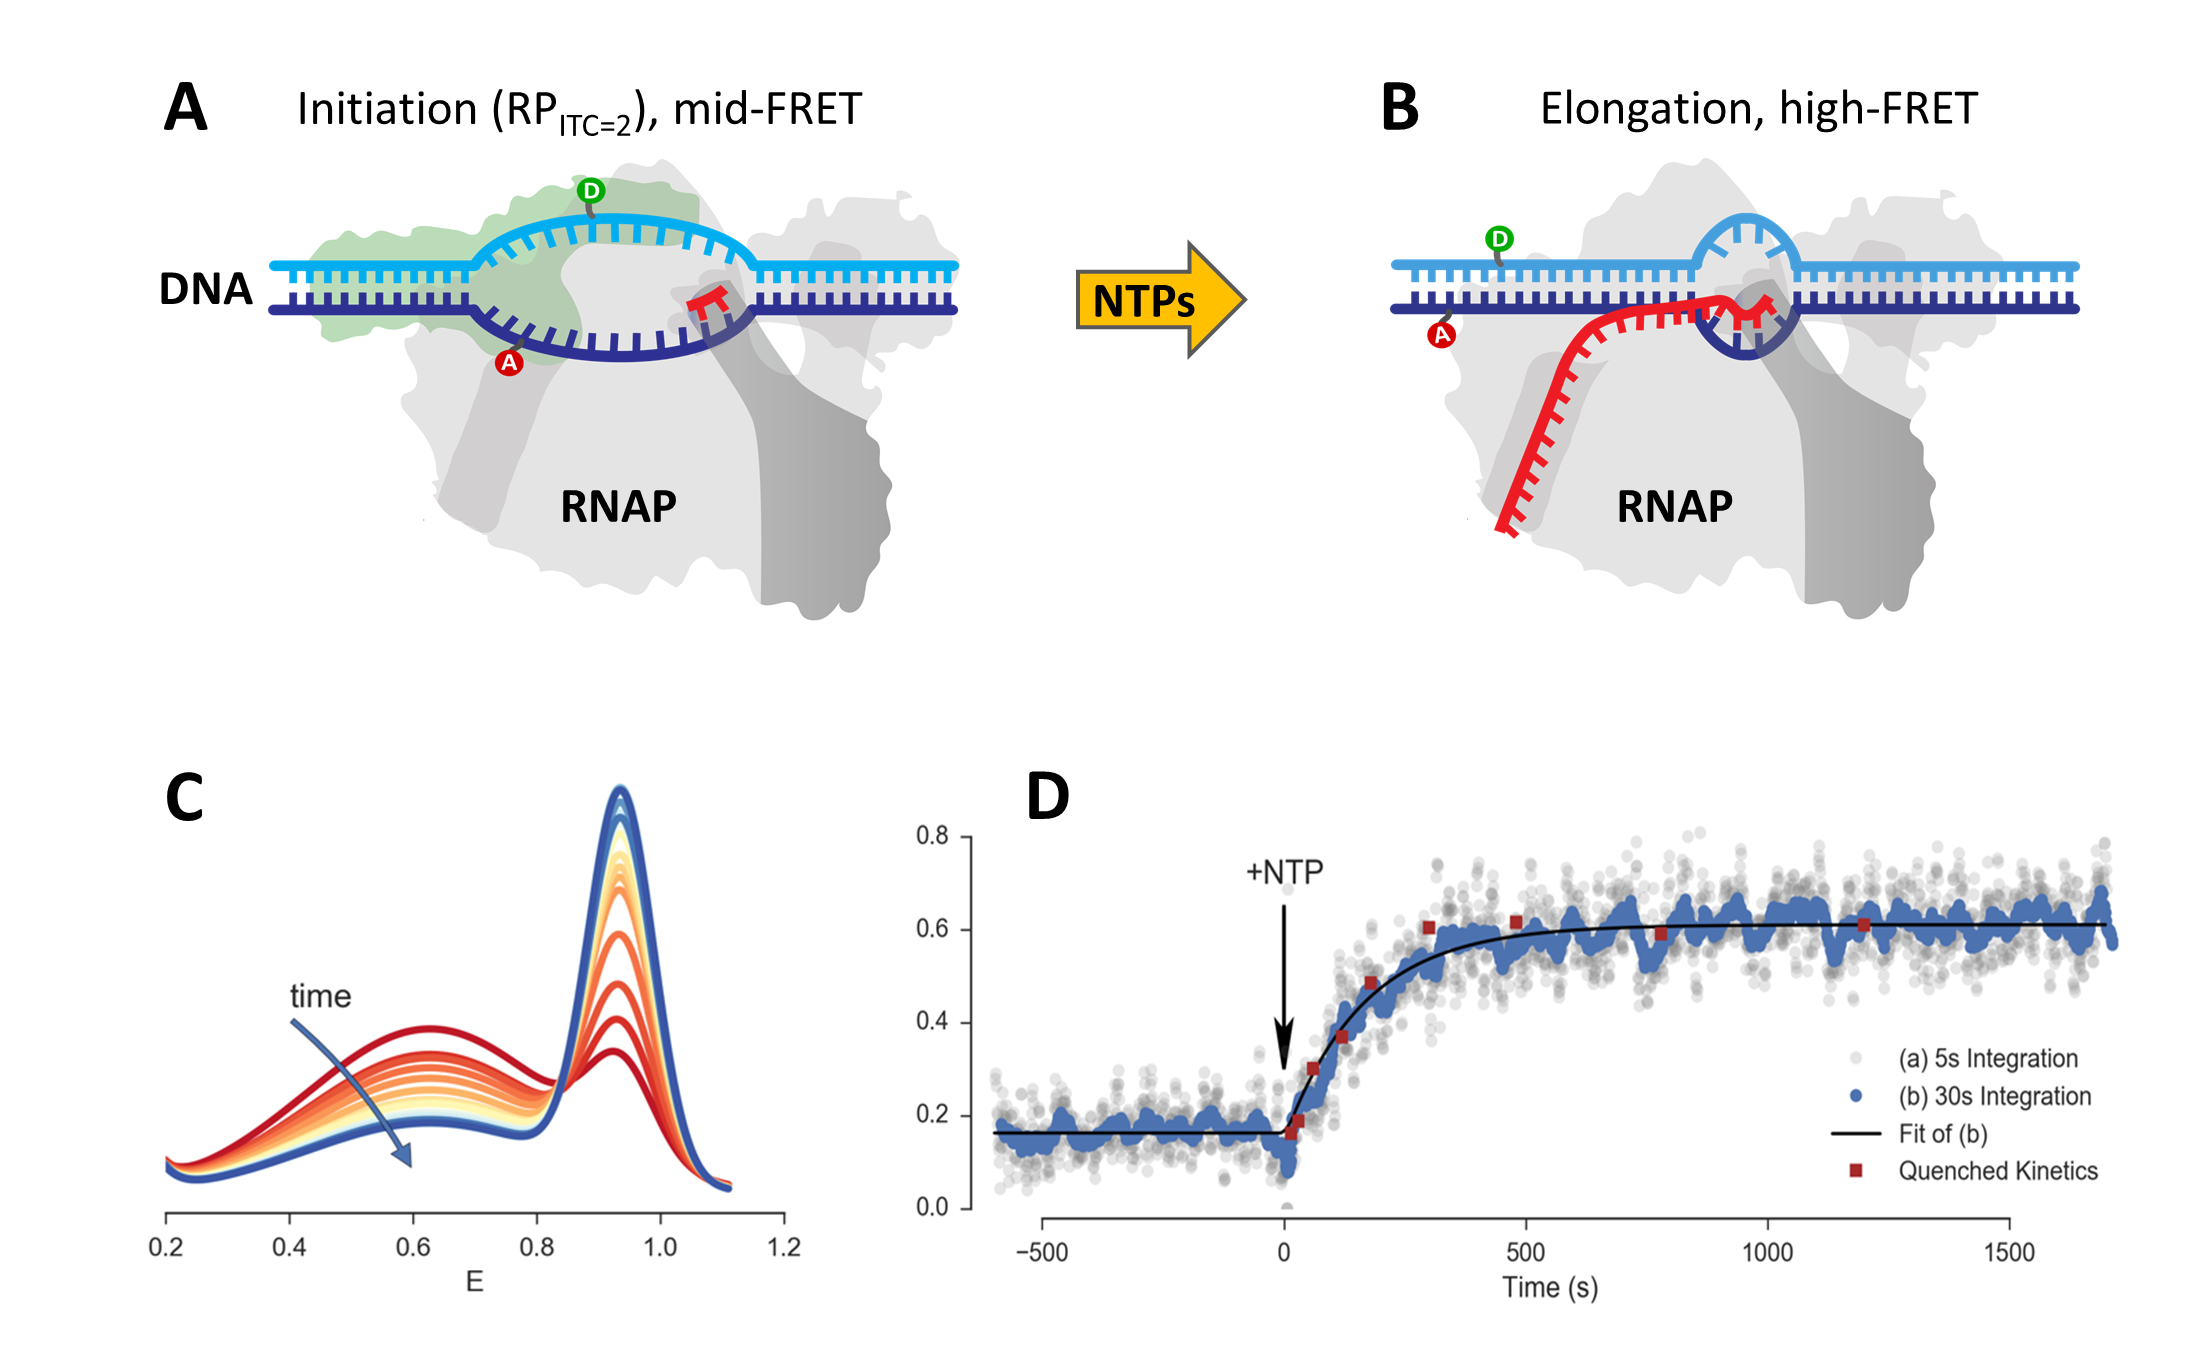
\includegraphics[width=\textwidth]{chapters/figures/RNAP_kinetics.png}
\caption{\label{fig:RNAP_kinetics} 
RNAP kinetics study.
A) The RNAP-promoter initial transcribing complex ($RP_{ITC}$) is prepared with a stabilizing dinucleotide (red symbol) as the nascent RNA chain.
Complementary DNA strands are labeled at DNA promoter bases with donor (D, green, position -5) and acceptor (A, red, position -8) dyes. 
After formation of a transcription initiation bubble, the bases to which the dyes are conjugated
are separated, resulting in medium FRET. 
The initial state remains in stationary conditions until the addition of the four missing nucleotides (\ac{NTP}s, yellow arrow), which triggers transcription initiation and elongation. 
B) During elongation, the transcription bubble moves downstream (to the right), resulting in re-hybridization of the open-bubble at the promoter sequence, and a corresponding decrease in the D-A distance (\textit{i.e.} an increase in FRET efficiency).
C) Evolution of uncorrected FRET efficiency ($E_{PR}$) distributions as function of time.
The curves represent Gaussian fits of the $E_{PR}$ histograms using 30~s time windows.
D) Fraction of high FRET population obtained in the real-time kinetics measurement (grey and blue dots).
Dots are computed as a function of time using either a 5~s (grey) or 30~s (blue) moving integration window.
The solid black curve is a single-exponential model fitted to the 30~s moving integration window.
Quenched kinetics data (red dots)~\cite{lerner_PNAS_2016}, normalized to fit initial and final values of
the real time kinetics trajectory, are also shown for comparison.
For more details on the analysis see the Jupyter notebook provided in Ingargiola \textit{et al.}, 2017~\cite{ingargiola_PLOS1_2016}.
Figure adapted from Ingargiola \textit{et al.}, 2017~\cite{ingargiola_PLOS1_2016}.
}
\end{figure}

\subsection{RNAP kinetics}
\label{sec:kinetics_analysis}

In this study, we investigated the initial stage of transcription using the 8-spot \ac{HT-smFRET} setup~\cite{ingargiola_PLOS1_2016}. 
The reaction was initiated by manually adding a complete set of nucleotides. 
In practice, this meant pipette mixing the \ac{NTP}s into the solution while the sample was mounted on the microscope stage. 
After manual mixing, we continuously recorded smFRET bursts from diffusing single complexes in the solution. 
You can find detailed information about the experimental setup in the original 8-spot publication~\cite{ingargiola_PLOS1_2016}.

Data analysis was performed using procedures typically employed for steady-state or equilibrium measurements. 
These procedures included background estimation, burst search, and burst selection, with no corrections applied. 
The only difference was that the resulting bursts were grouped into different time windows, as explained below.

During the initial phase of the experiment before adding nucleotides, two sub-populations were identified, i) the $RP_{ITC=2}$ complex with medium FRET ($E_{PR} = 0.62$), and ii) the unbound \ac{dsDNA} with high FRET ($E_{PR} = 0.95$).
As anticipated, a fraction of free \ac{dsDNA} molecules (the aforementioned high FRET population), indistinguishable from the final population of molecules that had completed transcription, was present in the sample.
Following the addition of nucleotides, the faction of sub-populations was analyzed using 30~second time windows and shifting them in 1~second increments. 
This approach allowed quantification of the fractional occupancy of the resulting FRET sub-populations as a function of time, as illustrated in Figure~\ref{fig:RNAP_kinetics}C.

Figure~\ref{fig:RNAP_kinetics}D exhibits a first-order exponential kinetics pattern, characterized by $\tau \approx 172 \pm 17$ seconds.
Interestingly, data analyzed using a 5~second sliding window, depicted with grey dots in Figure~\ref{fig:RNAP_kinetics}D, display a similar trend, albeit with a lower signal-to-noise ratio. 
This finding underscores the importance of employing a larger number of sampling volumes to access shorter time scales. 

The observed kinetics of this experiment aligned with results obtained through an entirely independent method involving a series of quenched transcription reactions monitored using standard equilibrium \ac{smFRET} measurement in solution~\cite{lerner_PNAS_2016} (illustrated by the red dots in Figure~\ref{fig:RNAP_kinetics}D). 
The agreement between these studies validates the suitability of the \ac{HT-smFRET} approach for studying slow kinetics.

Furthermore, this study underscores a significant advantage of \ac{HT-smFRET}. 
The quenched kinetics assay, which necessitated 20 minutes per red dot in Figure~\ref{fig:RNAP_kinetics}D, resulted in a total acquisition time of $9 \times 20 = 180$ minutes. 
In contrast, the real-time kinetics assay conducted on the 8-spot setup required just 30 minutes of acquisition time (20~minutes if we stopped at the same point as the quench kinetics assay). 
This demonstrates the substantial reduction in experimental time afforded by \ac{HT-smFRET}.

However, the time resolution of this rudimentary approach, which involves manually adding and mixing reactants to trigger the reaction, is constrained by the dead-time associated with the mixing process itself, on the order of tens of seconds. 
To investigate even shorter time scales, it is necessary to combine this approach with faster microfluidic mixing techniques.

\section{HT-smFRET in microfluidic devices}
\label{sec:microfluidics}

\subsection{Introduction}
\label{sec:microfluidics_intro}

As previously suggested, the full potential of multispot \ac{SPAD} arrays becomes evident when they are integrated with microfluidic devices. 
In the following sections, we introduce three types of devices that facilitate various forms of \ac{HT-smFRET}:

\begin{enumerate}
\item Microfluidic \enquote{formulator} device,
\item Parallelized microfluidic device,
\item Microfluidic device based on hydrodynamic focusing.
\end{enumerate}

\begin{figure}
\centering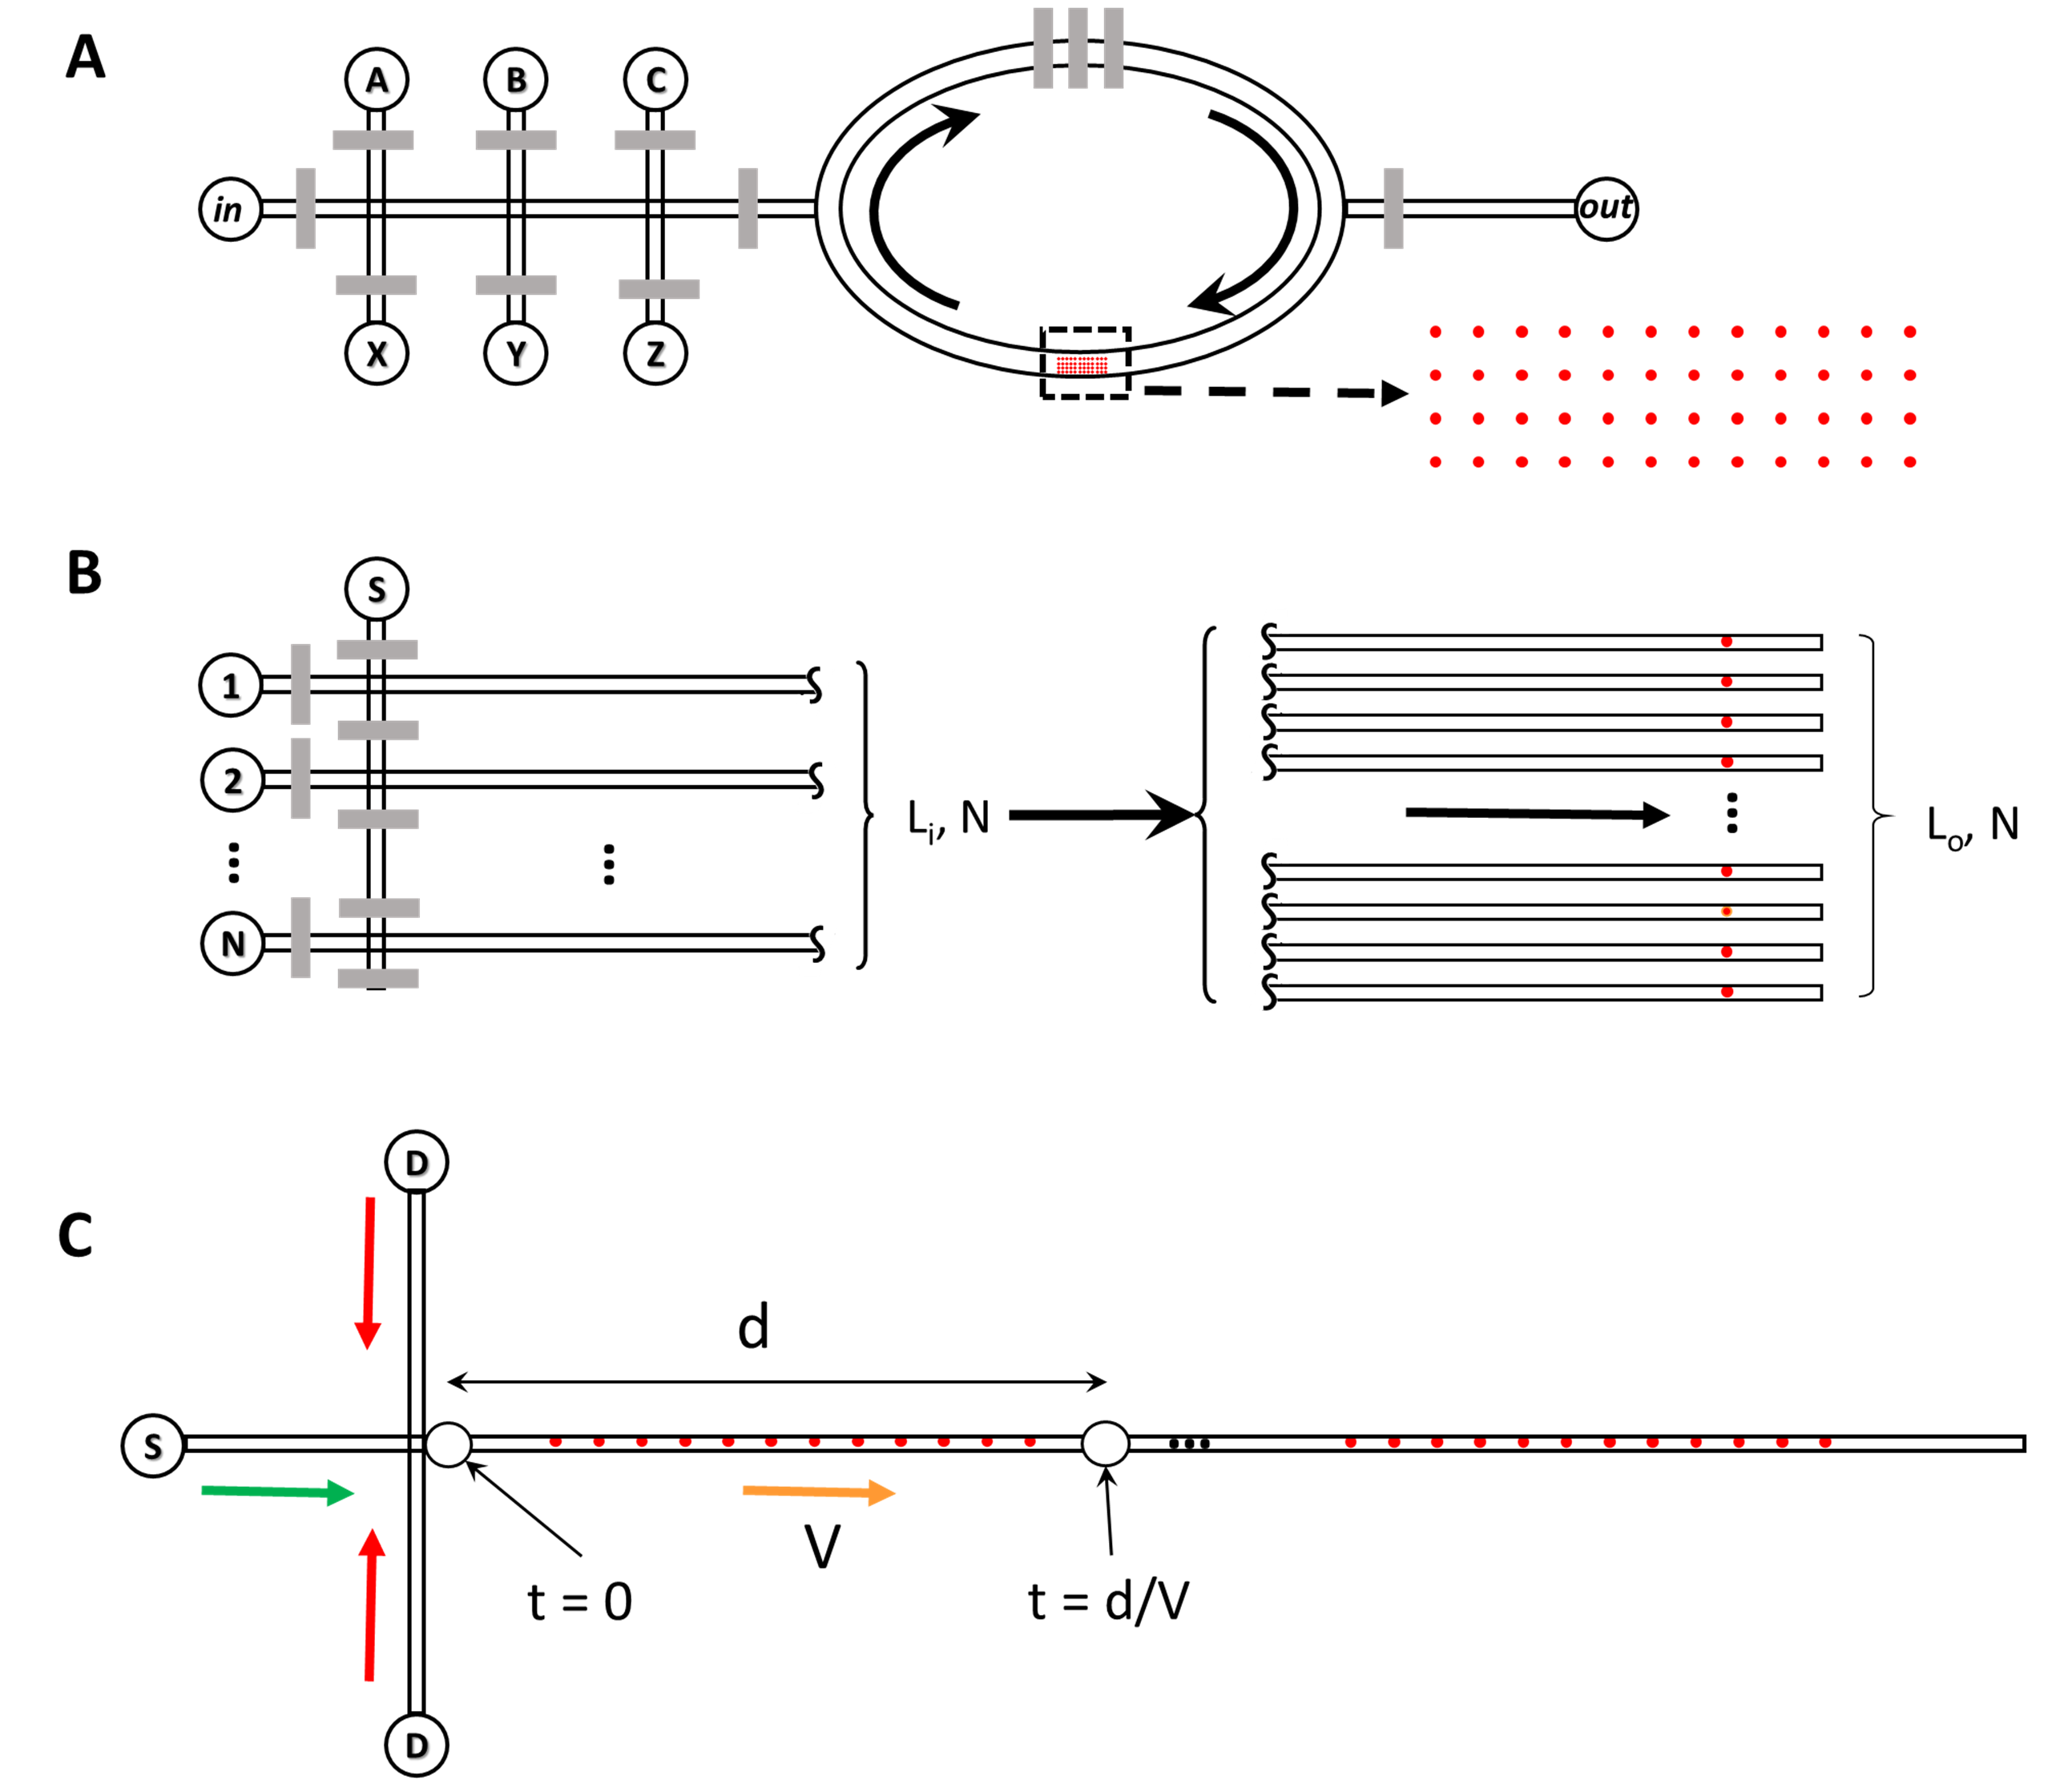
\includegraphics[width=0.8\textwidth]{chapters/figures/microfluidic_examples.png}
\caption{\label{fig:microfluidic_examples} Examples of possible \ac{SPAD} array and microfluidic combinations.
A) Formulator geometry: in a microfluidic formulator, several sample reservoirs (A, B, C, ..., X, Y, Z) are connected to an injection channel via programmable valves (grey rectangles), which allow precise injection of volumes ($pL$) of sample within a mixing region (ellipse). 
A peristaltic pump mechanism (top three grey rectangles) allows mixing of different sample aliquots within a few seconds.
Equilibrium measurements of the mixed sample can then be performed in an observation chamber (dashed rectangle) using a dense array of independent spots such as that described in section~\ref{sec:HT-smFRET_measurements_DNA}.
B) High-throughput screening geometry: a linear multispot \ac{SPAD} array combined with a multichannel microfluidic channel would allow high-throughput, parallel single-molecule detection, with applications in molecular screening and diagnostics. 
The channel separation on the inlet side ($L_i/N$) is much larger than their separation on the outlet side ($L_o/N$), set to match the excitation spot pitch.
C) Microfluidic mixer geometry: in a fast single-molecule microfluidic mixer, a sample (S) is rapidly mixed with another solution (D), plunging molecules quasi-instantaneously in a different environment, thus triggering a series of changes (conformation, chemical, or enzymatic reaction, etc.). 
A multispot setup with a linear illumination scheme and \ac{SPAD} array
would allow acquiring information from individual molecules at as many time points along the reaction coordinate in parallel, thus speeding up fast kinetic measurements. 
Figure reprinted from Segal \textit{et al}~\cite{segal_methods_2019}.
}
\end{figure}

The microfluidic \enquote{formulator} device, as illustrated in Figure~\ref{fig:microfluidic_examples}A, offers the capability of swift and precise mixing of small volumes of reactants (down to picoliters). 
This device enables prolonged measurements, sample flushing, and automated titration with flexibility for numerous repetitions. 
When applied to \ac{HT-smFRET} analysis, it enhances throughput beyond what was achievable in single-spot geometry experiments~\cite{kim_NM_2011}. 
Devices like the formulator opens up opportunities for rapid exploration of the equilibrium conformational dynamics of biomolecules and the investigation of how enzymatic activity is influenced by varying chemical conditions.

In contrast to the experiments performed on the formulator~\cite{kim_NM_2011}, where the measurement time required overnight data acquisition, \ac{HT-smFRET} has the potential to dramatically decrease the measurement time to the mixing time scale of this type of mixer, which is typically just a few seconds. 
For instance, if an 8-spot setup collects one data point within a 5~second acquisition time window (as described in Fig.~\ref{fig:RNAP_kinetics}), using our 48-spot setup would reduce the required acquisition time to achieve similar statistics to less than 1 second. 
While this time resolution is considerably faster than what can be achieved with a standard single-spot setup, it remains slower than what is attainable with a continuous flow mixer, which can reach millisecond time scales (as discussed in Section~\ref{sec:microfluidics}). 
Apart from speeding up data acquisition, reduced experiment duration offers other benefits, including minimized sample degradation and reduced setup drift across experiments.

A parallelized microfluidic approach, as illustrated in Fig.~\ref{fig:microfluidic_examples}B, involves each spot of a multispot setup probing a distinct sample. 
To achieve this, the device can comprise numerous independently accessible channels, possibly utilizing a microfluidic multiplexer. 
This configuration enables controlled mixing and probing of a common sample ($S$) with multiple probes ($1...~N$). 
However, the parallel geometry presents technical challenges, demanding precise alignment between the spot density, constrained by the field of view of a high numerical aperture microscope, and microchannel density, limited by the resolution of soft-lithography. 
Implementing this approach would likely necessitate custom-designed optics for larger \ac{SPAD} arrays compared to those discussed in this article.

Microfluidic hydrodynamic focusing, as depicted in Fig~\ref{fig:microfluidic_examples}C~\cite{knight_PRL_1998,lipman_science_2003,gambin_LoC_2010,wunderlich_NP_2013} achieves mixing rates several orders of magnitude faster than the formulator. 
This is accomplished by injecting a sample ($S$) into a cross-junction along with a \enquote{diluent} solution ($D$), causing the three input streams to mix in the outlet channel. 
Various geometries, such as the one described in Hamadani \textit{et al.}\cite{hamadani_BJ_2008}, can achieve the same outcome. 
In this setup, as long as the flow remains laminar, a thin slab of sample, $S$ $<<1~\mu$m, becomes focused between laminar streams of the surrounding diluent solution. 
Due to the narrow width of the sample slab, sample and solute molecules diffuse and mix on the timescale of microseconds to milliseconds ($\mu$s - ms). 
Beyond this \enquote{time 0} point within the mixer's primary channel, sample molecules evolve in a diluent environment as they flow along the main channel. 
The time $t$ since the start of the reaction is given by $t = d/V$, where $d$ represents the distance from the mixing region, and $V$ is the flow velocity.

Single-molecule measurements with hydrodynamic focusing have traditionally employed single-spot approaches, necessitating the accumulation of data one time-point at a time, which is both time-consuming and sample-intensive. 
However, adopting a linear \ac{SPAD} array geometry in combination with a linear illumination pattern, as demonstrated in the 8-spot publication~\cite{ingargiola_SPIE_2017}, would significantly expedite data acquisition in fast kinetics experiments of this kind. 
Additionally, it offers the exciting possibility of tracking the evolution of individual molecules along their reaction path.

Similar types of measurements have previously been demonstrated using cameras, achieving temporal resolutions ranging from approximately 100~$\mu$s~\cite{oikawa_SR_2013,oikawa_JPCB_2015} to 10~ms~\cite{fontana_LoC_2019}. 
In these setups, single molecules are either rapidly flowed ($>50$~mm/s) through a simple microfluidic channel and detected as streaks by an electron-bombarded camera~\cite{oikawa_SR_2013,oikawa_JPCB_2015}, or they are transported in very narrow channels at speeds compatible with single-molecule localization ($<1$~mm/s) and tracked using stroboscopic illumination~\cite{fontana_LoC_2019}.

Both of these approaches could be adapted for use with \ac{SPAD} arrays and fast single-molecule microfluidic mixers. 
In the first case, where fast flow exceeds 50~mm/s, it would result in very low photon counts per spot due to limited excitation intensity and the short transit time of each molecule through the detection spot. 
However, there would be a high likelihood of detecting the same molecule in consecutive spots along the flow direction, as the large flow velocity minimizes the effect of lateral diffusion. 
For example, for a spot separation of 2~$\mu$m a temporal resolution of approximately 40~$\mu$s could be achieved. 
While individual single-molecule time traces generated under these conditions may offer limited information due to the low signal-to-noise ratio, the cumulative statistical analysis of a large number of such time traces could provide unprecedented insights into single-molecule dynamics.

In the second case, where the flow velocity is less than 1~mm/s, the time resolution with identical spot separation would be reduced to more than 2~ms. 
However, the signal-to-noise ratio would remain compatible with single time-point \ac{smFRET} measurements. 
In this scenario, the likelihood of capturing the same molecule in consecutive spots would be limited by diffusion. 
Nevertheless, conducting cumulative analysis on a substantial number of such short trajectories would still offer valuable insights into single-molecule dynamics.

\subsection{Proof of principle experiment}
\label{sec:microfluidics_experiment}

Following the characterization of the enhanced throughput of the 48-spot setup, we transitioned to a proof-of-principle experiment that would demonstrate the measurement of a flowing sample on the \ac{HT-smFRET}-PAX setup, as described in Section~\ref{sec:HT-smFRET_measurements}.

In this experiment, I utilized a basic microfluidic device, which consisted of a single channel and a viewing chamber with dimensions $L \times W \times H = 3.6$~mm $\times  320~\mu$m $\times 10~\mu$m. 
This device was fixed to a glass coverslip for meausuing on the microscope.
Inlet and outlet holes, approximately 0.5~mm in diameter, were created using a biopsy punch and connected to 20 gauge Tygon tubing via 23 gauge stainless steel pins.

To drive the flow, I connected the outlet tubing to a luer-locking 23 gauge syringe tip, which in turn was linked to a 1~mL Norm-ject syringe mounted in a programmable syringe pump (NE-1000 Multi-Phaser, New Era Pump Systems, NY). 
I injected a 500~pM sample of doubly-labeled dsDNA (ATTO~550 and ATTO~647N separated by 5~bp, as described in Lerner \textit{et al.}, 2017~\cite{lerner_transcription_2017}) into the inlet Tygon tubing. 
I then used the syringe pump to pull this sample into the chip, maintaining a constant flow rate of approximately 10~$\mu$L/hr.

For measurements in the absence of flow, I used an average output power of 300~mW for the 532~nm and 628~nm lasers. 
However, in the presence of flow, it was necessary to increase the laser powers to compensate for the shorter residence time of molecules in the excitation spots. 
Specifically, I used a total laser power of 500~mW for the 532~nm laser and 800~mW for the 628~nm laser, where the average power at 628~nm due to \ac{PAX} alternation was 400~mW. 

\subsection{Flow characterization by CCF analysis}
\label{sec:microfluidics_CCF}

The flow velocity can be determined by calculating the \ac{CCF} of the intensity signals recorded at two positions separated by a distance $d$ along the flow direction, which is known as the two-beam cross-correlation method~\cite{brinkmeier_AC_1999}. 
The normalized 2D \ac{CCF} is expressed as:

\begin{equation}
\label{eqn:CCF_flow}
CCF_{flow}(t) = \left[N \left(1+\frac{t}{\tau_D} \right) \right]^{-1}
\exp \left[ -\frac{V^2}{w_{xy}^2}\frac{\left(t - \tau_F\right)^2}{1+t/\tau_D}\right] 
\end{equation}

\noindent
where $\tau_D$ is the diffusion time across each excitation-detection volume,
assumed to be Gaussian in the $x-y$ plane with waist $w_{xy}$:

\begin{equation}
    \label{eqn:tau_d}
    \tau_D = \frac{w_{xy}^2}{4D}
\end{equation}

\noindent
and where $D$ is the diffusion constant, $V$ is the flow velocity and $\tau_F = d/V$ is the time it takes a molecule to traverse the distance between two adjacent spots.

In the measurement geometry shown in Figure \ref{fig:flow_analysis}A, there are several pairs of spots with different separations:

\begin{itemize}
    \item 36 pairs of spots separated by $d_0 = 5.4~\mu$m
    \item 24 pairs of spots separated by $2 \times d_0$
    \item 12 pairs of spots separated by $3 \times d_0$
\end{itemize}

Pairs of spots at an angle with respect to the flow direction could also be considered for this analysis. 
Since these pairs are equivalent, we averaged the \ac{CCF} corresponding to the same separation but to different pairs. 
This averaging process results in the curves shown in Figure~\ref{fig:flow_analysis}B.

In the presence of flow, characteristic peaks at time scales $\tau_{F_i}$ (where $i = 1, 2, 3$) were visible in both channels along the direction of the flow. 
These time scales were approximately $21~m$s, $41~m$s, and $61~m$s. Importantly, these peaks were not observed in the opposite direction of flow, which was as expected. 
In the absence of flow (Figure~\ref{fig:flow_analysis}C), no peaks were detected, which was also expected.

The translation time between consecutive spots corresponded to an average flow velocity $V_{meas}$ of approximately $257~\mu$m/s. 
This measured velocity was slightly different from the programmed flow rate and channel dimensions ($V_{theo} \sim 309~\mu$m/s). 
The small discrepancy is consistent with the expected behavior at a slightly off-center vertical position within the channel, considering the quasi-parabolic dependence of the velocity profile with the vertical position within the channel, as discussed in Wunderlich \textit{et al.}, 2014~\cite{wunderlich_LOC_2014}.

\begin{figure}
\centering
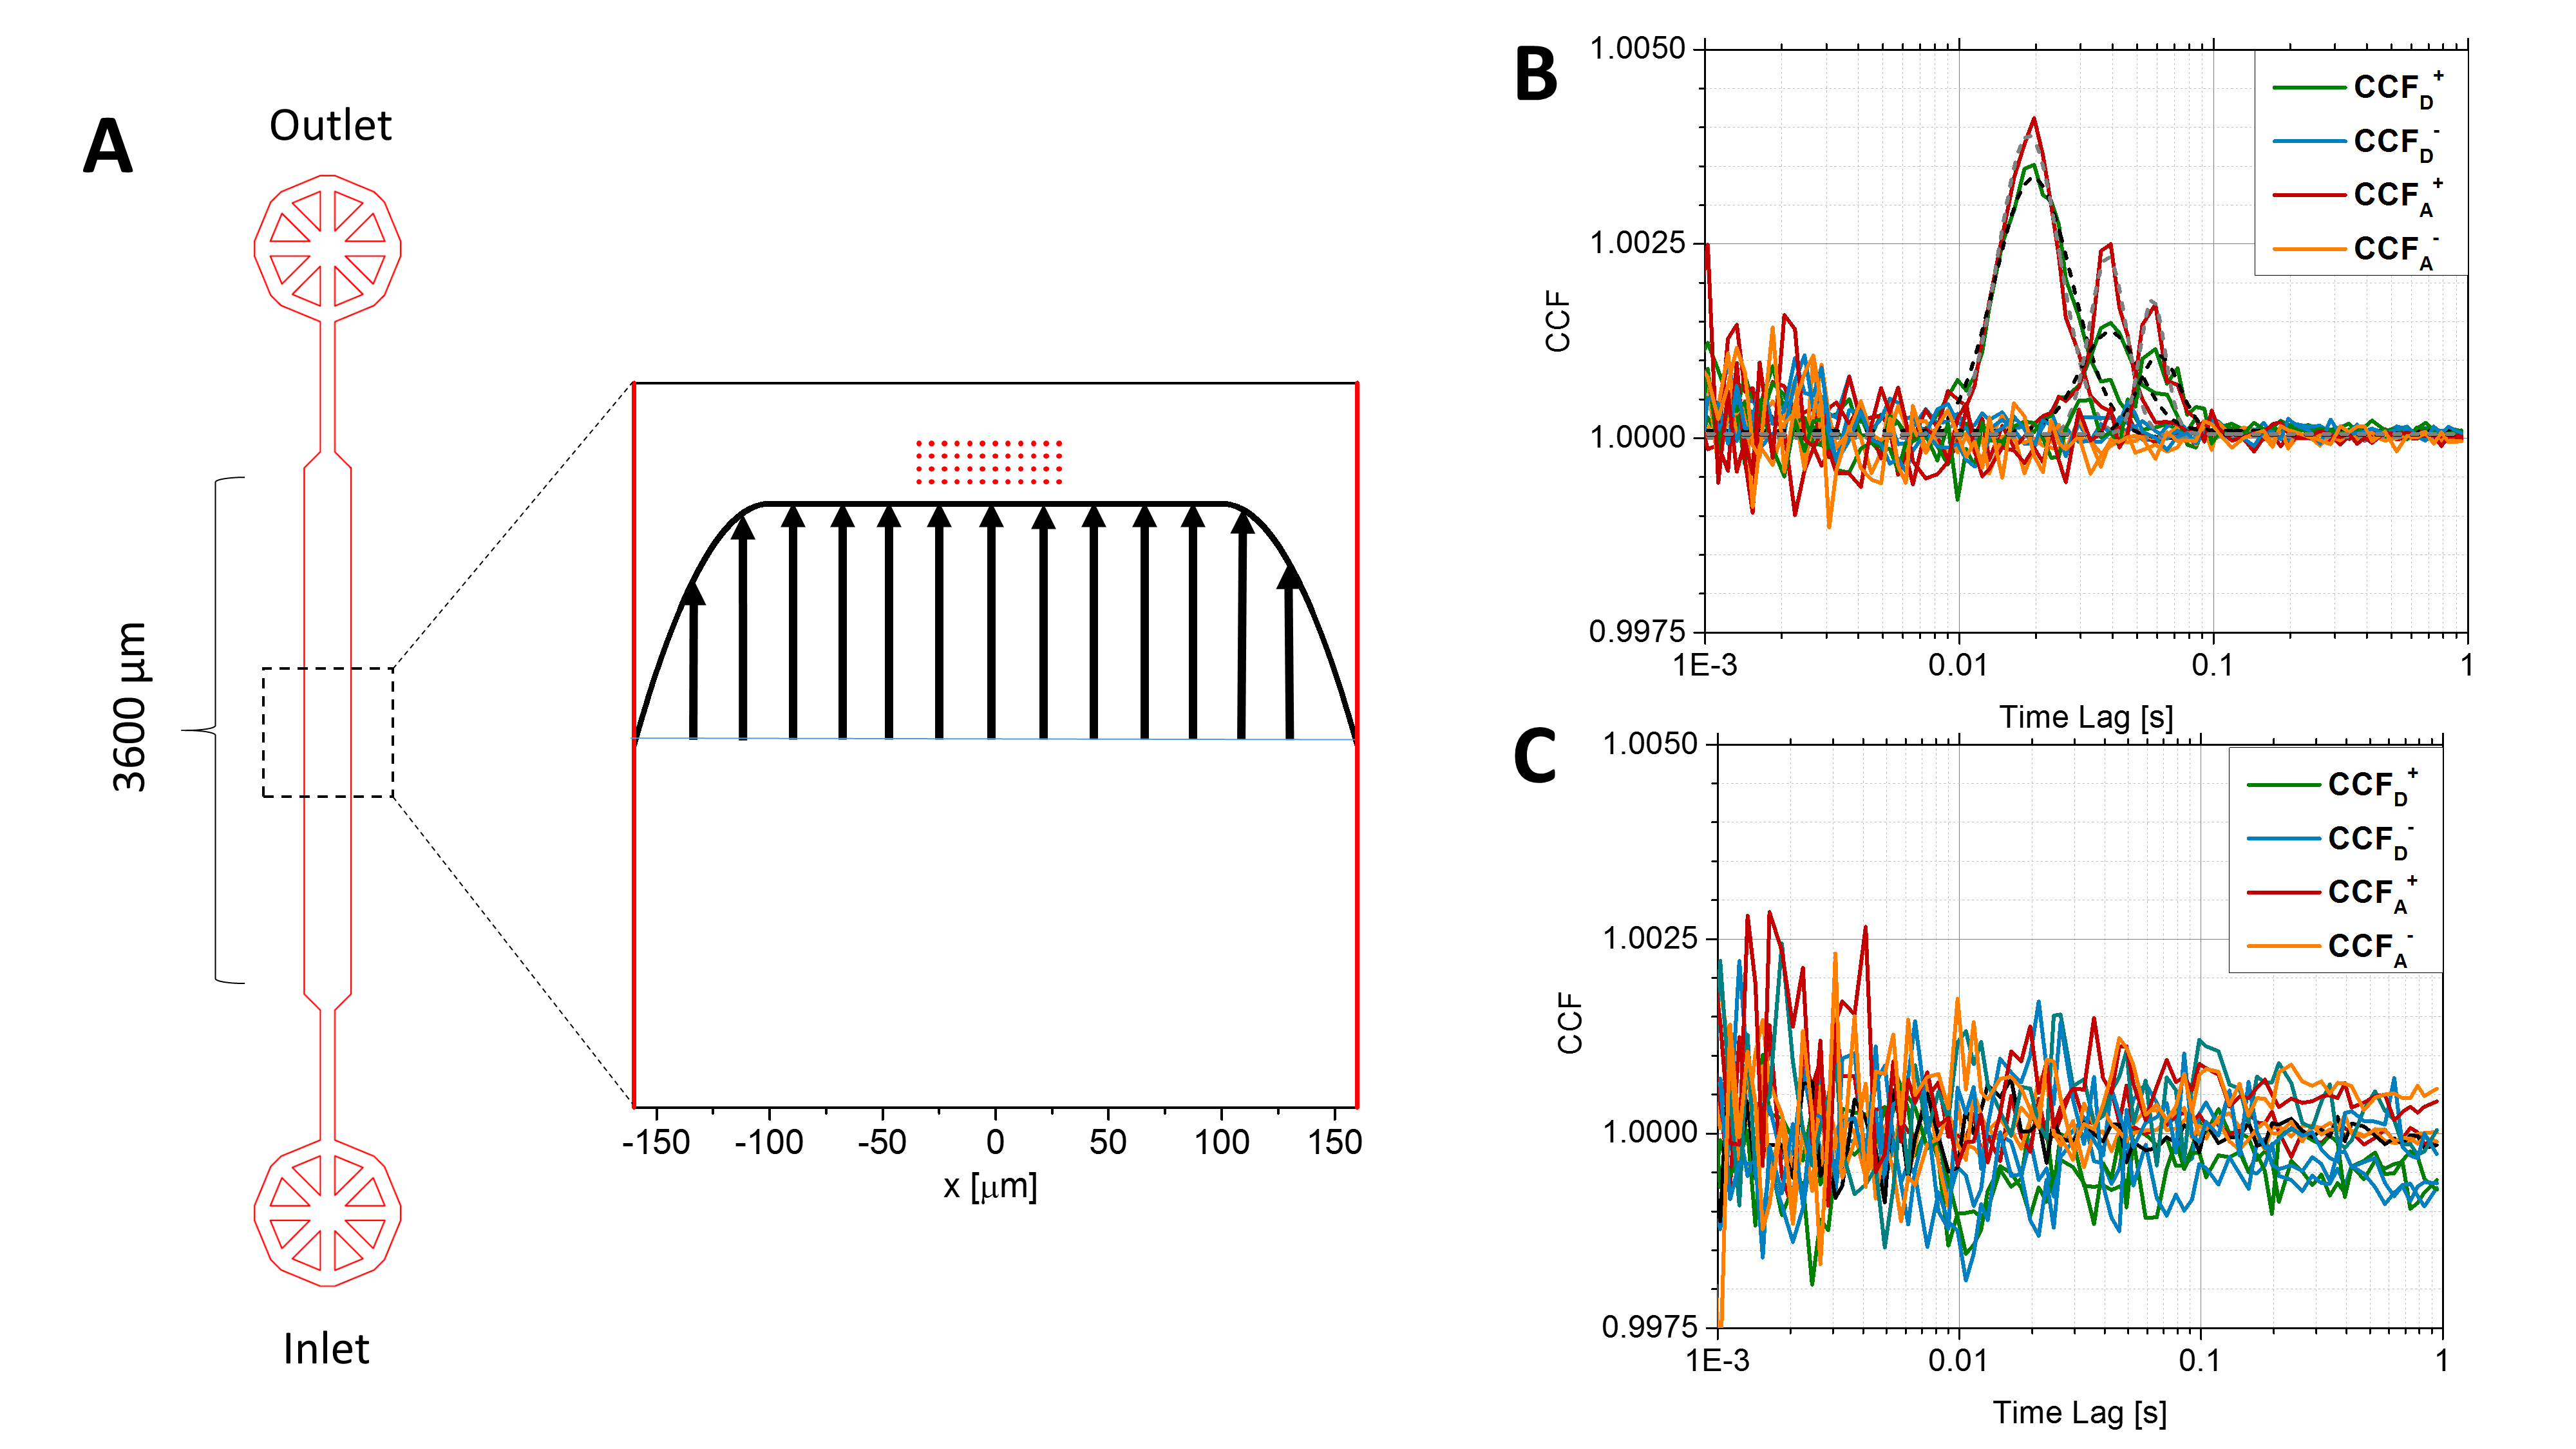
\includegraphics[width=\textwidth]{chapters/figures/flow_analysis.png}
\caption{\label{fig:flow_analysis} 
\ac{HT-smFRET} in a microfluidic chip.
A: Measurements were performed in the center of a simple microfluidic chamber in which a single-molecule sample of 
doubly-labeled \ac{dsDNA} \ac{lacCONS} promoter (ATTO~550 at -3~\ac{bp} and ATTO~647N at -8~\ac{bp} with respect to the transcription start site~\cite{lerner_transcription_2017}) was flown at a constant flow velocity, $V$. 
The 48-spot excitation pattern (red dots, width $\sim60~\mu$m, pitch distance $d_0 = 5.4~\mu$m) was located in the center of, and perpendicularly to the $320~\mu$m-wide channel, in a region where the velocity profile (schematically represented by the black curve and parallel arrows) is approximately constant in the $x-y$ plane and parabolic along the vertical direction (not shown).
B: The average \ac{CCF}s of adjacent spots (distance $d_1 = d_0$), spots separated by $d_2 = 2 \times d_0$
or $d_3 = 3 \times d_0$ along the direction of the flow, calculated for both donor (green) and acceptor (red) detection channels over the first 200~s, exhibit a clear peak around $\tau_{F_i} \sim$ 21, 41 and 61~ms, as fitted using Eq.~\ref{eqn:CCF_flow} (grey and black dashed curves).
No such peak is visible in the corresponding average \ac{CCF}s computed in the reverse direction (blue and orange curves) or in the absence of flow. 
Fits of the \ac{CCF} curves with Eq.~\ref{eqn:CCF_flow} yield an average flow velocity $V$ {$=253 \pm 6~\mu$}m/s, or a transit time across a single spot $\tau_T \sim 3 \omega_xy/V \sim 3~ms \sim ~11 \tau_D$, where the diffusion time $\tau_D \sim 268~\mu$s was obtained from a fit of the average donor channel \ac{ACF}s.
Datasets used for this figure as well as ALiX notebooks and associated files used for analysis can be found in the Figshare repository~\cite{figshare_repo_2019}.
Reprinted from Segal \textit{et al.}~\cite{segal_methods_2019}.
}
\end{figure}

\section{HT-smFRET in a simple microfluidic device}
\label{sec:smFRET_microfluidics}

The measured velocity falls within the range of flow velocities commonly used for \ac{smFRET} analysis in microfluidic mixers~\cite{lipman_science_2003, wunderlich_NP_2013}. 
This range of velocities was chosen to ensure that there is a sufficient transit time for accumulating an adequate number of photons during a single-molecule burst for analysis.

However, it is important to note that the velocity used in this experiment was much slower than the velocities typically employed in high-throughput single-molecule detection setups, where flow velocities can reach several centimeters per second. 
Achieving such high flow velocities requires significantly higher excitation powers to generate a detectable single-molecule signal~\cite{horrocks_AC_2012}.

To evaluate the impact of flow on single-molecule burst properties, we conducted a comparison between $E_{PR}-S$ histograms. 
These histograms were aggregated from data acquired over all 48 spots. 
Initially, I collected data for the sample under conditions of free diffusion, and then repeated the measurements in the presence of flow, with higher excitation power, as explained earlier. 
Both sets of measurements were recorded for 200~seconds. 
The resulting histograms (Figure~\ref{fig:ES_flow_noflow_comparison}) revealed that, although the relative proportions of donor-only and FRET bursts differed due to varying excitation intensities, their individual characteristics in terms of $E_{PR}$ and $S$ remained unchanged.

\begin{figure}
\centering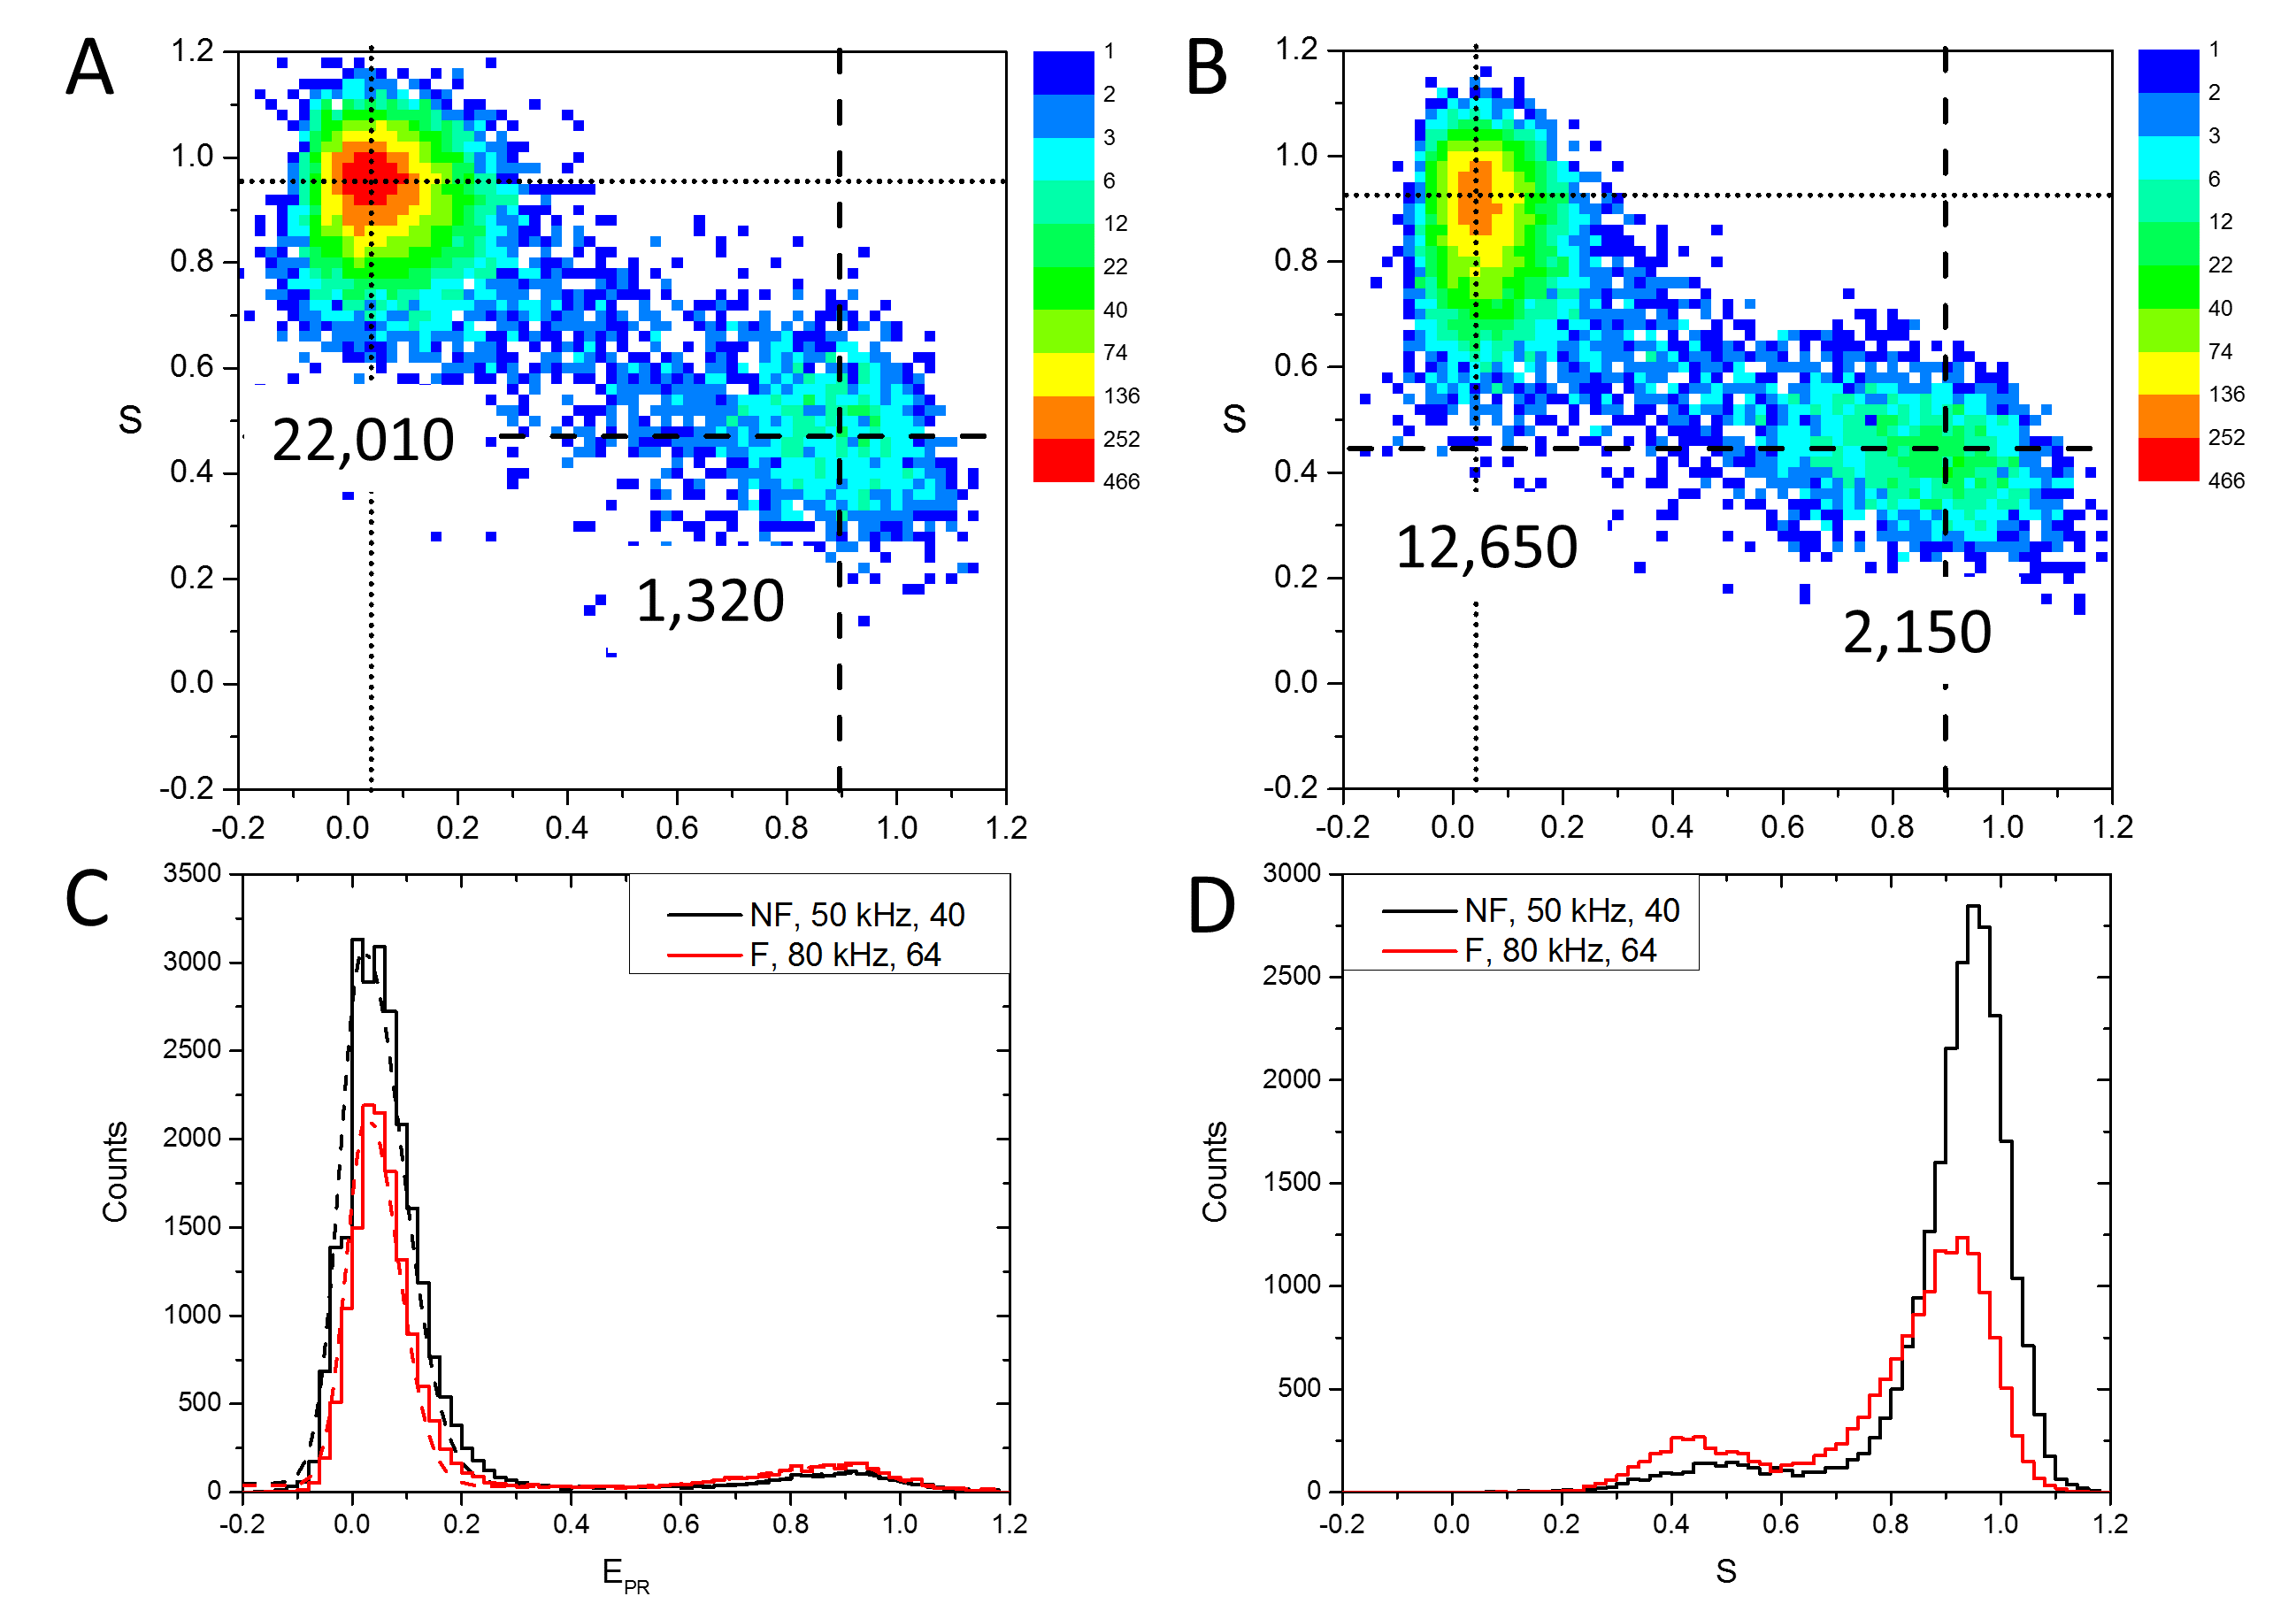
\includegraphics[width=\textwidth]{chapters/figures/ES_flow_noflow_comparison.png}
\caption{\label{fig:ES_flow_noflow_comparison} 
A,B: Comparison of the $E_{PR}-S_u$ histograms
of a dsDNA FRET sample in the absence (A) or in the presence (B) of flow.
The diffusion only (no flow or NF) dataset, recorded with lower excitation powers (by a factor $\sim1.6$), was analyzed with a lower rate threshold ($r_m \geq 50$~kHz) for burst search and a lower burst size threshold ($\overline{F} \geq 40$) for burst selection, than the dataset recorded with flow (F), for which $r_m \geq 80~$kHz $= 50 \times 1.6$, $\overline{F} \geq 64 = 40 \times 1.6$, in order to obtain comparable number of bursts for analysis.
The numbers next to each sub-population (top-left: donor-only, middle-right: FRET) correspond to the estimated integral under each peak as discussed in C. The $E_{PR},S_u$ location of the donor-only and FRET populations is identical in both experiments. 
Note that the color scale is logarithmic.
C: Projected $E_{PR}$ histograms for the no flow (NF, black) and flow (F, red) measurements. 
Dashed curves correspond to fits with a model of asymmetric Gaussian with tilted bridge described by Eq.~\ref{eqn:two_bridged_peaks_model} in section~\ref{sec:E_S_histogram}. 
The integral under each peak, given by Eq.~\ref{eqn:AG_peak_integral} provides an estimate of the number of bursts in each sub-population, as reported in A \& B.
D: Projected $S_u$ histograms for the no flow (NF, black) and flow (F, red) measurements.
Details of the analysis can be found in the different notebooks:
\texttt{ALiX Notebook, XX, APBS, m = 10, Rmin = YY kHz, Smin = ZZ.rtf} where XX = Flow or No Flow,
YY = 50 or 80, ZZ = 40 or 64, and associated files in the Figshare repository~\cite{figshare_repo_2019})
Figure reproduced from Segal \textit{et al.}~\cite{segal_methods_2019}.
}
\end{figure}

To compensate for the influence of different excitation powers, we implemented specific criteria during burst search and selection. 
The burst search used the rate criterion $r_m > R_{min}$ (see Eq. \ref{eqn:local_rate}) and the burst selection criterion $\overline{F} > \overline{F}_{min}$.
These criteria are adjusted in proportion to the excitation power. 
For example, the donor laser excitation power is directly related to the burst peak count rates in the $D_{ex}D_{em}$ photon stream, as shown in Figure~\ref{fig:flow_burst_peak_r_D_D_48_spots}.

The observed increase in burst rate due to flow indicates that the throughput, which represents the number of bursts recorded per unit time, can be significantly enhanced even with moderate flow rates. 
This concept has been previously demonstrated in single-spot setups~\cite{horrocks_AC_2012}.
Furthermore, in contrast to diffusion-only measurements where a burst in a given spot might correspond to the same molecule diffusing in and out of the confocal volume, in the presence of flow each burst in a spot corresponds to a different molecule. 
Consequently, the resulting statistics can be directly translated into true sample concentration characteristics, eliminating the uncertainty associated with the stochastic nature of the number of bursts per molecule detected in diffusion-only experiments.

In this proof-of-principle experiment, analysis of statistics like burst size or burst duration was challenging due to the different excitation powers used in both measurements. 
However, a meaningful comparison can be made by examining the burst peak count rates of the donor-only and acceptor-only populations, as these rates scale with the excitation powers employed in each experiment.

These findings strongly emphasize the promise of integrating \ac{HT-smFRET} with microfluidics. 
However, it is worth noting that several trade-offs will require deeper investigation in future studies.
For example, one potential trade-off to consider is the relationship between flow velocity and burst numbers. 
Initially, increasing the flow velocity would lead to higher burst numbers. 
However, as the translational transit time ($\tau_D$) decreases with higher flow velocity, it may eventually lead to lower burst peak count rates. 
This could result in a decrease in the number of detected bursts (and a lower signal-to-noise ratio) unless compensation is made through adjustments in burst search and selection criteria, as well as increased excitation power, as demonstrated in previous studies~\cite{horrocks_AC_2012}.

Increased excitation power can lead to increased photobleaching, especially in mixer geometries where the same molecule may traverse several spots successively.
This continuous excitation for extended periods, particularly with linear illumination and detection geometry, can accelerate photobleaching~\cite{eggeling_AC_1998,eggeling_JPCA_2006,kong_JACS_2007}.
However, the ability to track the same single molecule across successive spots could offer exciting opportunities to study rapid conformational dynamics as a reaction evolves. 
This suggests a balance between higher excitation power for increased burst rates and the potential for increased photobleaching when designing experiments under flowing conditions.

